\documentclass[../../main]{subfiles}
\begin{document}

\subsection{Points of Interest}
\label{ss:final-poi}

A point of interest (\textit{poi}), as described earlier, is a tuple composed by a descriptive name, latitude, longitude, address (obtained through geocoding the latitude and longitude), a website URL and a phone number (if available), a category (\textit{restaurants}, \textit{sport}, \textit{leisure}) of the place.
Users can see their points of interest in the main screen of the application, the map, as markers.
Markers in the map have different colours based on their category, in order to differentiate them.
Users can create a new \textit{poi} by tapping on the map or by inserting an address into the search bar on top of the screen\footnote{It is actually disabled because it works through Google's Places API, which is not free. Of course, it can be enabled by giving an API key linked to an account with credits in it.}.
If users open the \textbf{Points of interest} screen from the main menu, they can see the complete list of their \textit{pois} and from here they can view their details, share them or start the navigation to them.
In the following pictures we can see the \textbf{Points of interest} screen and the dialog that appears onto the map when creating a new \textit{poi}.
\begin{figure}[H]
    \centering
    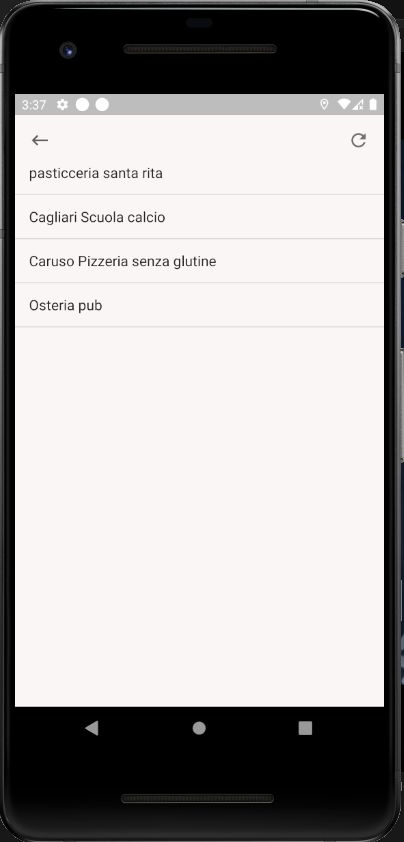
\includegraphics[width=0.4\textwidth]{images/app/poi/poi_overview}
    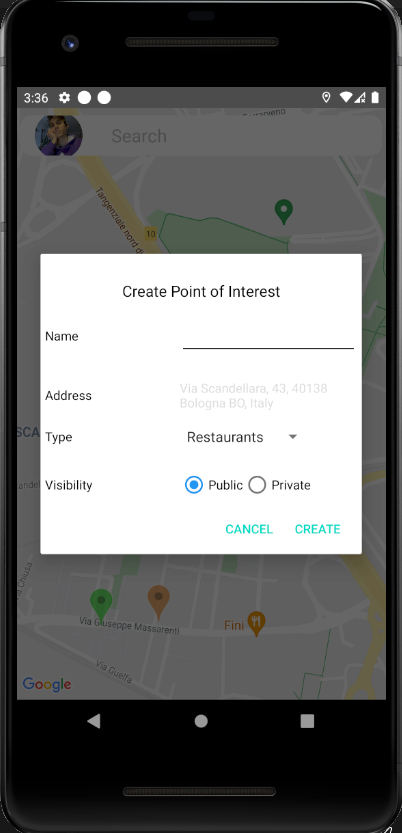
\includegraphics[width=0.405\textwidth]{images/app/poi/creazione_poi}
    \caption{On the left, the \textbf{Points of interest} screen. On the right, the dialog for creating a \textit{poi}.}
\end{figure}
\noindent
By clicking on a \textit{poi} it is possible to see its detail, share it and start the navigation, like we mentioned above.
\begin{figure}[H]
    \centering
    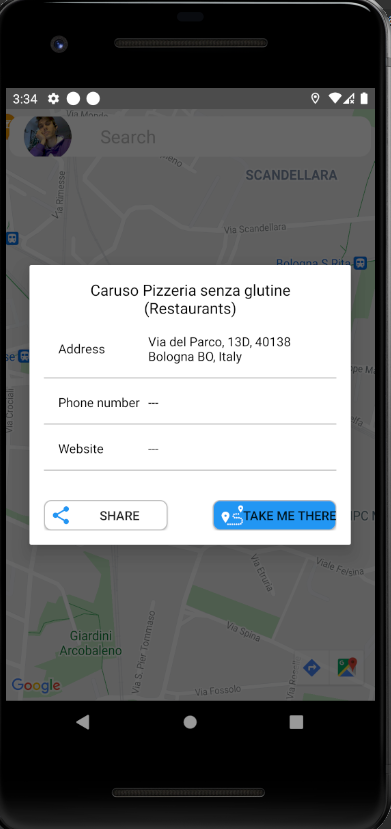
\includegraphics[width=0.4\textwidth]{images/app/poi/poi_map_detail}
    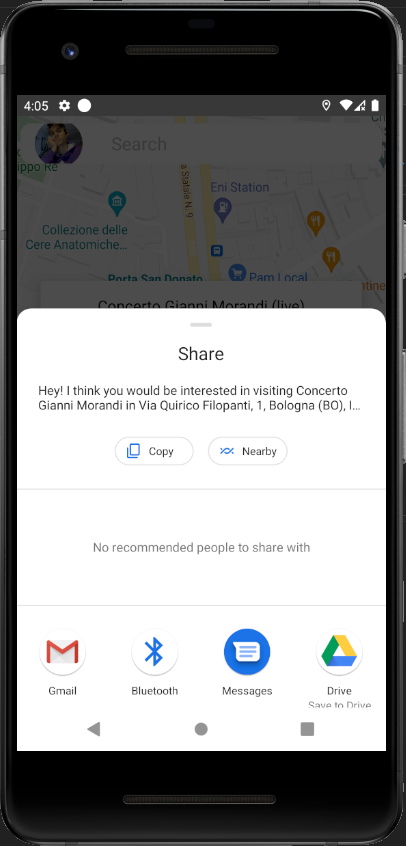
\includegraphics[width=0.41\textwidth]{images/app/share}
    \caption{On the left, the dialog to look at the detail of a \textit{poi}. On the right, the sharing interface for a \textit{poi}.}
\end{figure}
\end{document}